
%\newgeometry{top=1in,left=1.27in,right=2cm,bottom=1in}
\chapter{INTRODUCTION}

\par
\indent Online social networks provide new ways to generate and consume information.
Traditionally, people get information from either online news portals or blogs. But after
the advent of social networking sites like Facebook, Twitter, Google+, etc., people started
to receive information from these social networking sites. These sites are also used by
people to share the information they have across the network. They share the events that
happened in their own lives or events which they heard from someone else.
Micro-blogging websites have evolved to become a source of varied kind of information.The process of computationally categorizing opinions determine the writer's attitude towards a particular topic or product.

In this report, Twitter has been chosen as a medium to collect information from the users.
Twitter has been chosen due to the fact that most of the Twitter contents are public and
tweets are good indicators of user interests.Twitter has a combination
of features of both micro-blogging and social networking.
Twitter generates a vast amount of sentiment rich data in the form of tweets, status updates, blog posts etc.Sentiment analysis of this user generated data is very useful in knowing the opinion of the crowd.Using twitter's data and tools , this project aims in analyzing the interests of users.The interests of the user are obtained and output is projected in the form of graphs or pie charts.
Automatic identification of user interest from social media has gained much attention in recommendation systems and diverse ways of ad generation.
\vspace{1cm}
\section{MOTIVATION}
\par
\indent Due to the extensive use of social networking and micro-blogging sites, a vast data is generated.This huge amount of data contains useful information that can be used for various analysis and prediction.The unstructured nature of big data makes it difficult for analysis.Thus efficient learning algorithms can be employed for the analysis.
\vspace{1cm}
\section{OVERVIEW}
\par
\indent
 32 percentage of all Internet users are using Twitter.Twitter is an online social networking service that enables users to send and read short 280-character messages called "tweets".The three main difficulties in analysing social media contents are.
 \begin{itemize}
	\item[1 :]{Time Sensitivity \\Social networking site users post real time updates- movies, games, politics.Opens a large arena to know about the user's interest.For example:- users may not be interested in a movie which was released  several months ago, but due to a friend's recommendation,users   may be  interested in   a  movie irrespective of the release date.
Time sensitivity in social media data poses these  issues.}
	\item[2 :]{Short Length\\Social media sites restrict the length of the content posted by the users.Twitter allows user to post only content of length 280 characters.Processing these short texts poses a challenges to the text analytics method.Require lots of words to perform statistical analysis, which is missing in the case of social media text.}
	\item[3 :]{Unstructured Phrases\\Social media texts are unstructured compared to the traditional text.Text can be ungrammatical and cannot be fitted into the traditional semantics of text.Users can coin new terms or abbreviations which are not present in traditional text documents.eg: How r u?.Irrelevant contexts are written in one single text which makes it difficult to identify the domain. 


}
\end{itemize}

\chapter{REQUIREMENT ANALYSIS}
\section{User Interface}
\par
\indent 
The user interface implements a GUI which provides the user to provide inputs to the system in order to receive the required outputs. GUI is implemented as a web-app where the HTML and CSS scripting are used .  The input from the GUI is processed internally by the program and displays the corresponding output in the web page as a pie-chart.
\paragraph{}
\indent 
\textbf{FLASK:} \\
Flask which is python framework , is used as an integration tool for the backend with the front end web page. Flask is called a micro framework because it does not require particular tools or libraries. It has no database abstraction layer, form validation, or any other components where pre-existing third-party libraries provide common functions. However, Flask supports extensions that can add application features as if they were implemented in Flask itself. Extensions exist for object-relational mappers, form validation, upload handling, various open authentication technologies and several common framework related tools. Extensions are updated far more regularly than the core Flask program.Flask is also easy to get started with as a beginner because there is little boilerplate code for getting a simple app up and running. 
\\ \\
\textbf{Input:}
\begin{itemize}
\item The interface provides a feature to input a the required user's twitter-handle to filter his latest 3200 tweets loaded from the Twitter API.
\item The interface also provides a facility to input a keyword (probably hashtag)
and a geographical place with a radius which filters out the tweets regarding the keyword in that area.
\end{itemize}
\textbf{Output:}
\begin{itemize}
\item The user interests generator web page provides a pie-chart which describes his area of interest . The number of tweets and the percentage of interest he has in each given topic is displayed.
\item The geo-based tweet analysis of displays the percentage of positive , negative and neutral tweets of a product/event in and around the radius specified by the user.
\end{itemize}

\section{Functional Requirements:}
In Software engineering and systems engineering, a functional requirement defines
a function of a system or its component. Functional requirements may be calculations,
technical details, data manipulation and processing and other specific functionality that
define what a system is supposed to accomplish.
\subsection{Tweet Collection:}
The primary requirement of this project is the availability of tweets of a user or of a hash tag. Twitter provides developers with 1 percentage of its total data .REST API is used to read or write tweet data. OAUTH is used to authenticate the users
and Twitter applications. When an application requests for a tweet data, Twitter sends the
response in JSON format . There is a rate limit window of 15 minutes. Only 15 requests
can be made in this 15 minute window.Response data that is received from Twitter contains tweet text, list of hash-tags, list of
mentions, re tweet count, URLs, time zone, description about the user, geo-location, etc.,
Using these data from Twitter, various types of analysis could be made which could
provide deep insights about the user.For many years, Twitter has limited the use of third-party applications accessing the service by implementing a 100,000 user limit per application. Since August 2010, third-party Twitter applications have been required to use OAuth, an authentication method that does not require users to enter their password into the authenticating application.
\\
\textbf{TWEEPY:}\\
Python is great language for all sorts of things. Very active developer community creates many libraries which extend the language and make it easier to use various services. One of those libraries is tweepy. Tweepy is open-sourced library and enables Python to communicate with Twitter platform and use its API.The current version of tweepy is 1.13. It was released on January 17, and offers various bug fixes and new functionality compared to the previous version. The 2.x version is being developed but it is currently unstable so a huge majority of the users should use the regular version.
\paragraph{}
Tweepy supports accessing Twitter via Basic Authentication and the newer method, OAuth. Twitter has stopped accepting Basic Authentication so OAuth is now the only way to use the Twitter API.
Upon registering to REST API it provides the developers with 4 keys-
\textit{consumer key} \textit{consumer secret} \textit{access token} \textit{access token secret}.
The consumer key and the consumer secret are used for OAUTH handling whereas the acces token and the access token secret are used for setting access.\\
The main difference between Basic and OAuth authentication are the consumer and access keys. With Basic Authentication, it was possible to provide a username and password and access the API, but since 2010 when the Twitter started requiring OAuth, the process is a bit more complicated.OAuth is a bit more complicated initially than Basic Auth, since it requires more effort, but the benefits it offers are very lucrative:
\begin{itemize}
    \item Tweets can be customized to have a string which identifies the app which was used.
    \item It doesn’t reveal user password, making it more secure.
    \item It's easier to manage the permissions, for example a set of tokens and keys can be generated that only allows reading from the timelines, so in case someone obtains those credentials, he/she won’t be able to write or send direct messages, minimizing the risk.
    \item The application doesn't reply on a password, so even if the user changes it, the application will still work.
\end{itemize}
Although the documentation for tweepy is a bit scarce and doesn't have many examples, the fact that it heavily relies on the Twitter API, which has excellent documentation, makes it probably the best Twitter library for Python, especially when considering the Streaming API support, which is where tweepy excels. Other libraries like python-twitter provide many functions too, but the tweepy has most active community and most commits to the code in the last year.
\subsection{Geo-Coder}
Geopy is a Python 2 and 3 client for several popular geocoding web services.

It makes it easy for Python developers to locate the coordinates of addresses, cities, countries, and landmarks across the globe using third-party geocoders and other data sources.

Geopy is tested against CPython (versions 2.7, 3.4, 3.5, 3.6), PyPy, and PyPy3. It does not and will not support CPython 2.6.
Each geolocation service that one might use, such as Google Maps, Bing Maps, or Yahoo BOSS, has its own class in geopy.geocoders abstracting the service’s API. Geocoders each define at least a geocode method, for resolving a location from a string, and may define a reverse method, which resolves a pair of coordinates to an address. Each Geocoder accepts any credentials or settings needed to interact with its service, e.g., an API key or locale, during its initialization.
ocators’ geolocate and reverse methods require the argument query, and also accept at least the argument exactly one, which is True. Geocoders may have additional attributes, e.g., Bing accepts user location, the effect of which is to bias results near that location. geolocate and reverse methods may return three types of values.
\paragraph{}The tweets of a hash-tag in a particular place needs to be obtained to identify its market value. This is done by providing the latitude and the longitude of a the required place to REST API as input. Since user need not know the latitude and longitude of  a place , GEOPY library was used . Upon giving a place name as input it provides the latitude and longitude . This value is later used. geopy will log geocoding URLs with a logger name geopy at level DEBUG, and for some geocoders, these URLs will include authentication information. If this is a concern, one can disable this logging by specifying a logging level of NOTSET or a level greater than DEBUG for logger name geopy. geopy does no logging above DEBUG.
\subsection{Lexicon-Based dictionary:}
The Sentiment orientation dictionary(SO dcitionary) was used to get the sentiment of the words. The SO dictionary contains the sentiment words along with their respective polarities. The negator and intensifier dictionaries were also used.
\subsection{LIBSVM:}
LIBSVM and LIBLINEAR are two popular open source machine learning libraries, both developed at the National Taiwan University and both written in C++ though with a C API. LIBSVM implements the SMO algorithm for kernelized support vector machines (SVMs), supporting classification and regression. LIBLINEAR implements linear SVMs and logistic regression models trained using a coordinate descent algorithm. The goal is to help users to easily apply SVM to their applications. LIBSVM has gained wide popularity in machine learning and many other areas.It consists of many classification and regression algorithms.
The project uses linear kerneled SVM which was appropriate for text data.Even though there are lot of options the arguments should be tuned based on the size of the dataset and the number of features.
\section{Non-Functional Requirements:}
\begin{itemize}
\item \textbf{Performance:} The Twitter API will provide up-to-date information; limited only
by the rate of Twitter input.
The output should display the latest results at all times, and if it lags behind,
the user should be notified. The application should be capable of operating in the
background should the user wish to utilize other applications.

\item \textbf{Availability :}The software will be available at all times on the user’s device, as
long as the device is in proper working order . The functionality of the software
will depend on any external services such as uninterrupted Internet access that are
required.
\item \textbf{Security:} The software should never disclose any personal information of Twitter
users, and should collect no personal information from its own users. The use of
passwords and secret access and consumer keys will ensure private use of the Twitter API. The programs will be performed on a secured system to ensure maximum
security.
\item \textbf{ Maintainability:} The software should be written clearly and concisely. The code
will be well documented. Particular care will be taken to design the software mod-
ularly to ensure that maintenance is easy.
\item \textbf{Portability:} This software will be designed to run on any operating system that
has Python installed. To ensure the longevity of the software, the software is made
to be forward compatible with all OS and python updates.
\end{itemize}
\chapter{DESIGN}

The project was divided into 2 phases. The tasks under each of the phases were divided among the team members based on preferences and skill sets.
\\

\textbf{Phase 1}
\vspace{0.1cm}
\begin{itemize}
	\item[1 :]{Create an outline of the application, identify software needs, plan the application architecture}
	\item[2 :]{ Data Collection: Data consisted of tweets from 
	handles under the required categories or topics.}
	\item[3 :]{Text Mining: Creation of custom algorithms to mine the text from the tweets and remove noise}
	\item[4 :]{Creation of training and test files in the classifier library specific format and generating dictionaries.}
	\item[5 :]{Creation of algorithms to train and test the classifier with metrics for evaluation}
\end{itemize}

\textbf{Phase 2}
\vspace{0.1cm}
\begin{itemize}
	\item[1 :]{Measure effectiveness of the classifier using precision, recall and cross validation.}
	\item[2 :]{Refine the classifier using more training set and features.}
	\item[3 :]{Create the web interface running on a Flask server using Python script for users to view classified
tweets.}
	\item[4 :]{Code documentation and review.}

\end{itemize}
\section{ARCHITECTURE}
\begin{figure}[!ht]

\begin{tikzpicture}


    

\node [cloud, draw,cloud puffs=10,cloud puff arc=180, aspect=2, inner ysep=1em]at (0.5,0) (a) {Tweet Collect};



\node[block,below left =of a] (d) {PREPROCESSING1};
\node[block, below=  of d] (e) {REPRESENTING DATA};
\node[block,below = of e] (f) {MODEL GENERATION};
\node[block,below= of f] (g) {CLASSIFICATION};

\node[block,below right=of a] (h) {PREPROCESSING2};
\node[block,below=of h] (i) {SENTIMENT DICTIONARY};
\node[block,below=of i] (j) {SENTIMENT SCORE};

\node[block,below=of j] (c) {\textbf{OPINION ANALYSIS}};
\node[block,below=of g] (b) {\textbf{USER INTEREST GENERATOR}};
\node[block, below right=of b] (k) {DATA VISUALIZATION};

% \node[block] (e) at ([yshift=-2cm]$(b)!0.5!(c)$) {Gate};
%\node[draw,inner xsep=5mm,inner ysep=8mm,fit=(a)(b),label={130:A}](f){};
%\node[draw,inner xsep=5mm,inner ysep=8mm,fit=(c)(d),label={50:B}]{};
%\node[draw,inner xsep=5mm,inner ysep=6mm,fit=(b)(c)]{};
\draw[line] (a)-| (d);
 \draw[line,yshift=5mm] (a)-| (h);


\draw[line] (d) --(e);
\draw[line] (e) --(f);
\draw[line] (f) --(g);
\draw[line] (g) --(b);


\draw[line] (h) --(i);
\draw[line] (i) --(j);
\draw[line] (j) --(c);

\draw[line] (b) |-(k);
\draw[line] (c) |-(k);

%\draw[line] (b) --(d);
% \draw[line] (f.east) -- (c)node[pos=0.4,above]{flow};
% \draw[line] (c)-- (d);
%\draw[line] (e)-- ($(b)!0.5!(c)$);
\end{tikzpicture}
 \caption{Block diagram}
\end{figure}
\vspace{3cm}
\paragraph{}


The block diagram of the system architecture shown in Fig-3.1 explains the fundamental abstraction of the entire project.
The work has been viewed from 2 different perspectives. The first one is a personalized interest generator of a particular user. Hence the tweets pertaining to a particular user are only required to find his personal interests. Twitter provides access to user time-line of a given twitter-handle. The tweets are preprocessed to remove noise data. Preprocessing1 and Preprocessing2 indicates that the steps used in both these are different. Data once obtained must have a representation so that it can be easily be classified. The classifier creates a model which can be used for identifying the interest generator.  

The second view is about the public opinion about a particular event or a product. Hence in this level tweets pertaining to a particular topic are retrieved. Twitter API provides extensive services in query filtering based on user's requirement. The tweets obtained are preprocessed, but uses a slightly different approach here. A dictionary was primarily obtained which contained the polarity words and their values. This was used along with intensification's and conjunctive rules to obtain the polarity of a sentence/tweet. Hence each tweet was categorized positive negative or neutral base on this criteria.
\paragraph{}
\subsubsection{User Perspective}
\begin{figure}[!ht]
   
   
\begin{tikzpicture}

\node[block] (a) {WEB-APP};
\node[block,right = of a,xshift=3cm](b) {SERVER};
\node[draw,inner xsep=10mm,inner ysep=20mm,fit=(a)](c){};
\node[draw,inner xsep=10mm,inner ysep=20mm,fit=(b)](d){};

\draw[line] (a)--($(a.south)-(0,0.5)$) -| (b) ;
\draw[line] (b)--($(b.north)-(0,-0.5)$) -| (a);
%\draw[line] (Midi to CV.east) -| node[yshift=0em, xshift=-4em,fill=white]{Gate} (ADSR1.south);
\end{tikzpicture};
 \caption{Block diagram};
\end{figure};

The block diagram in the Fig-3.2 depicts the structure of the entire product from user's point of view.
The system consists of a web app which is used as a front end system. Users can communicate with the server using this interface.Flask, which is a python framework, is used for the purpose of integrating the interface and the server processes. The server after processing the retrieved data produces a result which could be visualized in the web page.

\section{STRUCTURE}
\subsection{Data Collection:}
\indent 
The first step in data flow is to stream data from twitter API in real time. Data in the form of raw tweets is acquired by using the python library tweepy. This library allows two modes of accessing tweets. One mode delivers a random sample of all the tweets streaming at a real time. Second mode delivers tweets that contain a specified keyword.
A tweet acquired by this method has a lot of raw information in it which we may not find useful for our particular application. It comes in the form of json file. Each tweet will have the following fields:
\begin{itemize}
    \item User Id
    \item Tweet Id
    \item Screen name
    \item Original tweet
\end{itemize}
Since this is a lot of information, only the needed information is filtered and rest is discarded. The process of removing unwanted information and formatting the tweets so that the next phase can effectively perform classification is known as pre-processing.

\begin{figure}
\begin{tikzpicture}

\node [cloud, draw,cloud puffs=10,cloud puff arc=120, aspect=2, inner ysep=1em] (a) {\textbf{Tweet Collect}};
\node[block,below =of a ] (b) {\textbf{TWITTER-API CALL}};
\node[block,below =of b] (d) {\textbf{PREPROCESSING}};

\node[block, below left =  of d ] (f) {WORDSET GENERATION};
\node[block, below right=  of d] (g) {DOCSET GENERATION};
\node[block, below right =  of f] (h) {LIBLINEAR REPRESENTATION};
\node[block,below left=of h] (i) {TRAINING};
\node[block, below=  of i] (e) {MODEL GENERATION};


\node[block,below right=of h] (m) {INTEREST GENERATOR};
\node[block,below=of m] (k) {CLASSIFICATION};
\node[block, below right=of e] (l) {VISUALIZATION};

% \node[block] (e) at ([yshift=-2cm]$(b)!0.5!(c)$) {Gate};
%\node[draw,inner xsep=5mm,inner ysep=8mm,fit=(a)(b),label={130:A}](f){};
%\node[draw,inner xsep=5mm,inner ysep=8mm,fit=(c)(d),label={50:B}]{};
%\node[draw,inner xsep=5mm,inner ysep=6mm,fit=(b)(c)]{};
\draw[line] (a)-- (b);
\draw[line] (b)-- (d);
\draw[line] (d)-| (f);
\draw[line] (d)-| (g);
\draw[line] (f)-| (h);
\draw[line] (g)-| (h);
\draw[line] (h)-| (i);
\draw[line] (h)-| (m);
\draw[line] (i)-- (e);
\draw[line] (m)-- (k);
\draw[line] (e)-- (k);
\draw[line] (k)|- (l);
%\draw[line] (db) --(d);
%\draw[line] (d) --(e);
%\draw[line] (e) --(f);
%\draw[line] (f) --(g);

%\draw[line] (c) --(h);% \draw[line] (b) -- (f.east);
%\draw[line] (h) --(i);
%\draw[line] (i) --(j);

%\draw[line] (g) |-(k);
%\draw[line] (j) |-(k);
%\draw[line] (b) --(d);
% \draw[line] (f.east) -- (c)node[pos=0.4,above]{flow};
% \draw[line] (c)-- (d);
%\draw[line] (e)-- ($(b)!0.5!(c)$);
\end{tikzpicture}
\caption{Block diagram}

\end{figure}
\subsection{Pre-Processing:}
\indent
Before using the Twitter data as training set, it was very important to pre-process the data to extract meaningful information. Twitter data consists of lots noise, which must be removed. Tweets are in an inconsistent format, they contain a lot of special characters, abbreviations, $@$ for mentions, \# for tags, misspelt words, URLs and exclamatory words. The following steps were done to remove noice data. 

\begin{itemize}

	\item	\indent [Rule 1 :]{Take only English language words. }
	\item\indent[Rule 2 :]{Remove all non-alpha numeric characters except hashtags and URLs .  }
	\item\indent[Rule 3 :]{ Remove stop words }

	\item\indent[Rule 4 :]{ Convert words to lower case which were not fully in upper case. }
	\item\indent[Rule 5 :]{Tokenize words using the whitespace.}
\end{itemize}

\subsection{Dictionary Generation:}
\indent 
Once the data has been obtained , the important step is to represent the data that could be  understandable by the algorithm . Since data has to be represented mathematically , the words have to converted into numerals.   Based on the application , two levels of dictionary are generated:
\begin{itemize}
    \item \textbf{Bag-of-Words Dictionary :}
    \indent 
    The Bag-of-Words is a Word-Id pair representation which converts each word into an id. This id is later referred in place of this word. After assigning each word an id, a tweet - word -category dictionary is generated. This represents a mapping of each word to a tweet and each tweet to a category. The category defines the labelling. The new tweet is assigned a category id 0. The rest of the categoryId's are assigned based on the categories.
   \paragraph{}
   \indent 
   Once dictionary has been made ,the next step is representation of the features.
   Liblinear representations have been used for it. The representation is an assignment of each tweet to a category which makes  labelling possible. The new tweets to be classified as label '0'. 
   
   \item \textbf{Sentiment orientation dictionary :}
   \indent
   The SO dictionary contains sentiment words along with their respective polarities.
   
   \item \textbf{Negator dictionary :}
   \indent
   The negator dictionary contains all the negator words and a flag 1 to indicate that it is negator.
   
   \item \textbf{Intensifier dictionary :} 
   \indent
   The intensifier dictionary consists of intensifiers and their degree of intensification expressed in percentage.
    
    
\end{itemize}

\subsection{Classifier:}
\indent 
Once the representation has been made , the data should  be passed to the classifier. The classifier used is SVM. A Support Vector Machine (SVM) is a discriminative classifier formally defined by a separating hyperplane. In other words, given labeled training data (supervised learning), the algorithm outputs an optimal hyperplane which categorizes new examples. In two dimentional space this hyperplane is a line dividing a plane in two parts where in each class lay in either side.
\paragraph{}
In machine learning, support vector machines (SVMs, also support vector networks[1]) are supervised learning models with associated learning algorithms that analyze data used for classification and regression analysis. Given a set of training examples, each marked as belonging to one or the other of two categories, an SVM training algorithm builds a model that assigns new examples to one category or the other, making it a non-probabilistic binary linear classifier (although methods such as Platt scaling exist to use SVM in a probabilistic classification setting). An SVM model is a representation of the examples as points in space, mapped so that the examples of the separate categories are divided by a clear gap that is as wide as possible. New examples are then mapped into that same space and predicted to belong to a category based on which side of the gap they fall.In addition to performing linear classification, SVMs can efficiently perform a non-linear classification using what is called the kernel trick, implicitly mapping their inputs into high-dimensional feature spaces.
.
\paragraph{}
Kernel Trick is used in SVM classification. The kernel trick simply finds the closeness of two given input data points .
SVM uses 3 kernels :
\begin{itemize}
	\item Linear
	\item Radial Basis Function(RBF)
	\item Polynomial
\end{itemize}

 \begin{figure}[!ht]
	\centering
	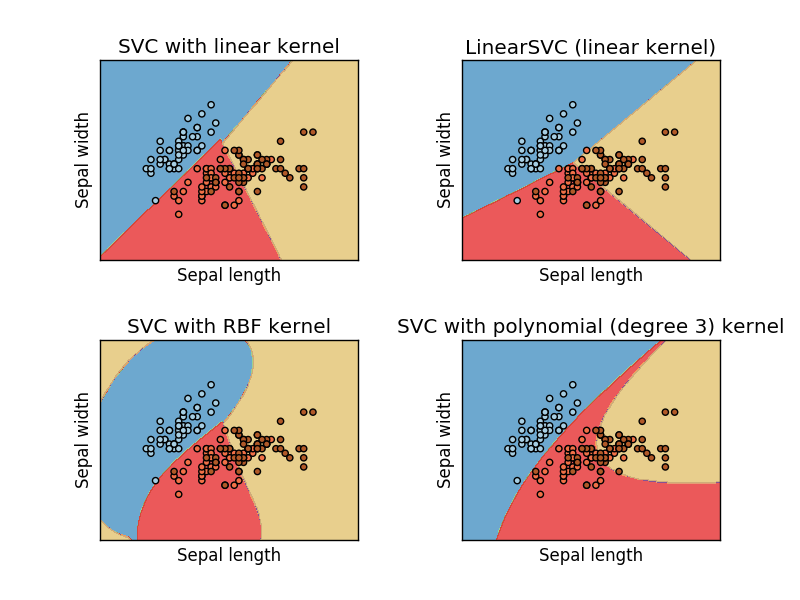
\includegraphics[width=0.9\linewidth]{svm_kernal.png}
	\caption{Different types of kernals}
	\label{fig:expression01}
\end{figure}

\paragraph{}
 In this project linear kernel has been used . Text classification problems usually uses linear kernel as these problenms are \textit(Linearly Seperable) problems. Moreover the features representations were sparse . The linear kernel trains comparitively faster than other kernel techniques.
 \paragraph{}
From the literature review, it was clear that in particular, the most  common technique in practice has been to build one-versus-rest classifiers  (commonly referred to as ”one-versus-all'' or OVA classification), and to choose  the class which classifies the test datum with greatest margin.
 \begin{figure}[!ht]
 	\centering
 	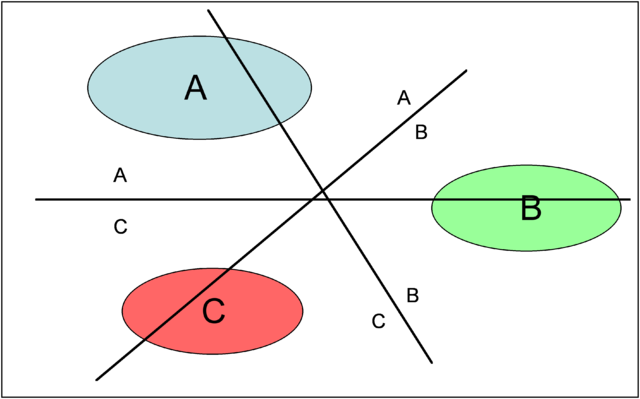
\includegraphics[width=0.9\linewidth]{svm_multi.png}
 	\caption{One vs all classifier}
 	\label{fig:expression01}
 \end{figure}
 \paragraph{}
 The one-vs rest(or one-vs.-all, OvA or OvR, one-against-all, OAA) strategy involves training a single classifier per class, with the samples of that class as positive samples and all other samples as negatives. This strategy requires the base classifiers to produce a real-valued confidence score for its decision, rather than just a class label; discrete class labels alone can lead to ambiguities, where multiple classes are predicted for a single sample.
 \paragraph{}
 
\subsection{Lexicon based approach for sentiment analysis :}
\indent
Opinion words are employed in many sentiment classification tasks. Positive opinion
words are used to express some desired states, while negative opinion words are used
to express some undesired states. There are also opinion phrases and idioms which
together are called opinion lexicon. 
Sentiment lexicons are lookup tables or dictionaries that map words to sentiment
scores. They provide a general method of sentiment analysis, and unlike machine
learning methods using classifiers, the lexicon can be applied across multiple do-
mains without retraining of the data. The lexicon based approach is faster than
the machine learning method.

%\node [block,below = of a] (e) {Sugar};
%\node[block,right=of a] (b) {Checkdam};
%\node[block,right= 3cm of b] (c) {Checkdam};
%\node[block,right=of c] (d) {Dam};

% \node[block] (e) at ([yshift=-2cm]$(b)!0.5!(c)$) {Gate};
%\node[draw,inner xsep=5mm,inner ysep=8mm,fit=(a)(b),label={130:A}](f){};
 %\node[draw,inner xsep=5mm,inner ysep=8mm,fit=(c)(d),label={50:B}]{};
%\node[draw,inner xsep=5mm,inner ysep=6mm,fit=(b)(c)]{};
%\draw[line] (a)-- (a|b);
%\draw[line] (b)-- (c);
%\draw[line] (e)-- (a);
% \draw[line] (b) -- (f.east);
% \draw[line] (f.east) -- (c)node[pos=0.4,above]{flow};
%\draw[line] (c)-- (d);
%\draw[line] (e)-- ($(b)!0.5!(c)$);

%\end{tikzpicture}
\section{ALGORITHM:}
\subsection{ALGORITHM FOR USER INTEREST}

\textbf{procedure preprocess(tweets:)}
\begin{enumerate}
    \item for each tweet in tweets:
    \begin{enumerate}
     \item for each word in tweet:
      \begin{enumerate}
          \item if word != 'A-Za-z1-9'* then
          \begin{itemize}
              \item remove the word.
          \end{itemize}
          \item if word == stopword.word()
          \begin{itemize}
              \item remove the word.
          \end{itemize}
          \item if(word.wordcount >12 and word.wordcount <3)
           \begin{itemize}
              \item remove the word.
          \end{itemize}
          
          
      \end{enumerate}
     \item Tokenize the words of the tweet.
     \item Add tweet to restweets.
    \end{enumerate}
    
    \item return restweets
\end{enumerate}
\paragraph{}

\textbf{procedure generate-dicts(tweet,catid) : }
\begin{enumerate}
  \item  categoryid = catid
  \item tweet-id = tweetid + 1
  \item for each word in tweet:
  \begin{enumerate}
      \item if word in wordset:
       \begin{enumerate}
           \item find word-id of word
           \item wordcount[word-id] += 1
           
       \end{enumerate}
       else:
        \begin{enumerate}
            \item increment word-id.
            \item assign word-id to word
        \end{enumerate}
        
  \end{enumerate}
  \item write each word and word-id to word dictionary.
  \item write category-id , tweet-id , word-id, weight to document dictionary
\end{enumerate}

\paragraph{}
\paragraph{}
\textbf{procedure librepresentation(categoryid):}
\begin{enumerate}
    \item read file docset.
    \item for each line in docset:
    \begin{enumerate}
        \item catid = line[0]
        \item tweetid = line[1]
        \item wordid = line[2]
        \item wght =  line[3]
        \item if catid == categoryid then:
        \begin{enumerate}
            \item add each tweet to libfile given the categoryid
        \end{enumerate}
        \item else:
        \begin{enumerate}
            \item add each tweet to libfile giving -1 as category. 
        \end{enumerate}
    \end{enumerate}
\end{enumerate}

\subsection{Algotithm for sentiment analysis}
\indent
\textbf{procedure sentiment(text)} \\
1. \indent preproc = preprocess(text) \\
2. \indent tokens = tokenize(preproc) \\
3. \indent for token in tokens  \\
4. \indent \indent prePol = currPol  \\
5. \indent \indent currPol = searchSoDictionary(token)  \\
6. \indent \indent if negFlag = 1 then \\
7. \indent \indent \indent if currPol != 0 then \\
8. \indent \indent \indent \indent currPol = currPol * -1 \\
9. \indent \indent \indent \indent negFlag = 0 \\
10.\indent \indent prevIntensifier = intensifierFlag \\
11. \indent \indent if intensifierFlag != 0 then \\
12. \indent \indent \indent if currPol != 0 then \\
13. \indent \indent \indent \indent currPol = currPol * intensifierFlag \\
14. \indent \indent \indent \indent intensifierFlag = 0 \\
15. \indent \indent currPol = currPol + prePol \\
16. \indent \indent if currPol = 0 then \\
17.	\indent \indent \indent negFlag = isNegator(token)  \\
18. \indent \indent \indent if negFlag = 0 then \\
19. \indent \indent \indent \indent intensifierFlag = getIntensification(token) \\
20. \indent return currPol \\

\indent
\textbf{procedure convertToDictionary()} \\
1. \indent wordFile = open SoTextFile for reading \\
2. \indent for entry in wordFile  \\
3. \indent \indent temp = split entry into word and value \\
4. \indent \indent key = temp.word \\
5. \indent \indent value = temp.value \\
6. \indent \indent if wordDict[key] = 0 then \\
7. \indent \indent \indent add to wordDict key, value \\

\indent
\textbf{procedure getIntensification(word)} \\
1. \indent checkFlag = checkValid(word) \\
2. \indent if checkFlag = True then \\
3. \indent \indent return intensifierDict[word] \\
4. \indent else \\
5. \indent \indent return 0

\indent
\textbf{procedure isNegator(word)} \\
1. \indent checkFlag = checkValid(word) \\
2. \indent if checkFlag = True then \\
3. \indent \indent return negDict[word] \\
4. \indent else \\
5. \indent \indent return 0 \\

\chapter{IMPLEMENTATION}
\indent 
\section{USER INTEREST GENERATOR}
\subsection{DATA COLLECTION}
\par In order to train the classifier 25000 tweets from each of the five categories were collected using Tweepy. To ensure that relevant tweets are collected , a  list of the top 15-20 most influential users for each category from Twitter’s recommended “Who to Follow”.We collected over 2000 tweets per user under each category into five separate text files. In addition to these steps mannual filtering were used.
\vspace{1cm}
\subsection{TEXT PROCESSING}
\par
\begin{itemize}

\item \textbf{Cleaning:}
\indent 
The greatest difficulty of twitter data is that it contains a large amount of unwanted symbols, smileys and special characters . These characters are difficult to parse and they may mean different in different contexts. They are difficult to interpret and must be removed. 

\item \textbf{Stopwords Removal:}
\indent 
The primary problem in most of the text documents is the occurrence of unwanted words which may be common in usage . But these words are usually unnecessary , since they do not provide any reference to a topic . Such words are to be removed. For eg:-'and','but',the.These words cannot directly express any kind of category words.
These words are commonly known as \textit{stopwords}. These words may occur very frequently in a document but does not imply any meaning.Thus they are removed in the primary stages of the project.

\item \textbf{Unwanted Keywords:}\indent
Micro-Blogging websites like Twitter are meant for expressing one's
opinions and expressions.Sometimes people use expressive keywords such as 'yeeeeaaaah' which may not be a keyword for interest classifier.  Eventhough such words provide sentiment they do not point a category. Thus these words were to be removed.After an analysis it was found that words having count greater than 12 and less than 3 were considered unwanted. Thus these words were elliminated.

\item \textbf{Tokenizing:}
\indent 
After the keywords are generated there is a need to split the words into individual tokens for representation . Tokenizing the words  into individual items are needed for the representation of data . 

\begin{figure}[!ht]
	\centering
	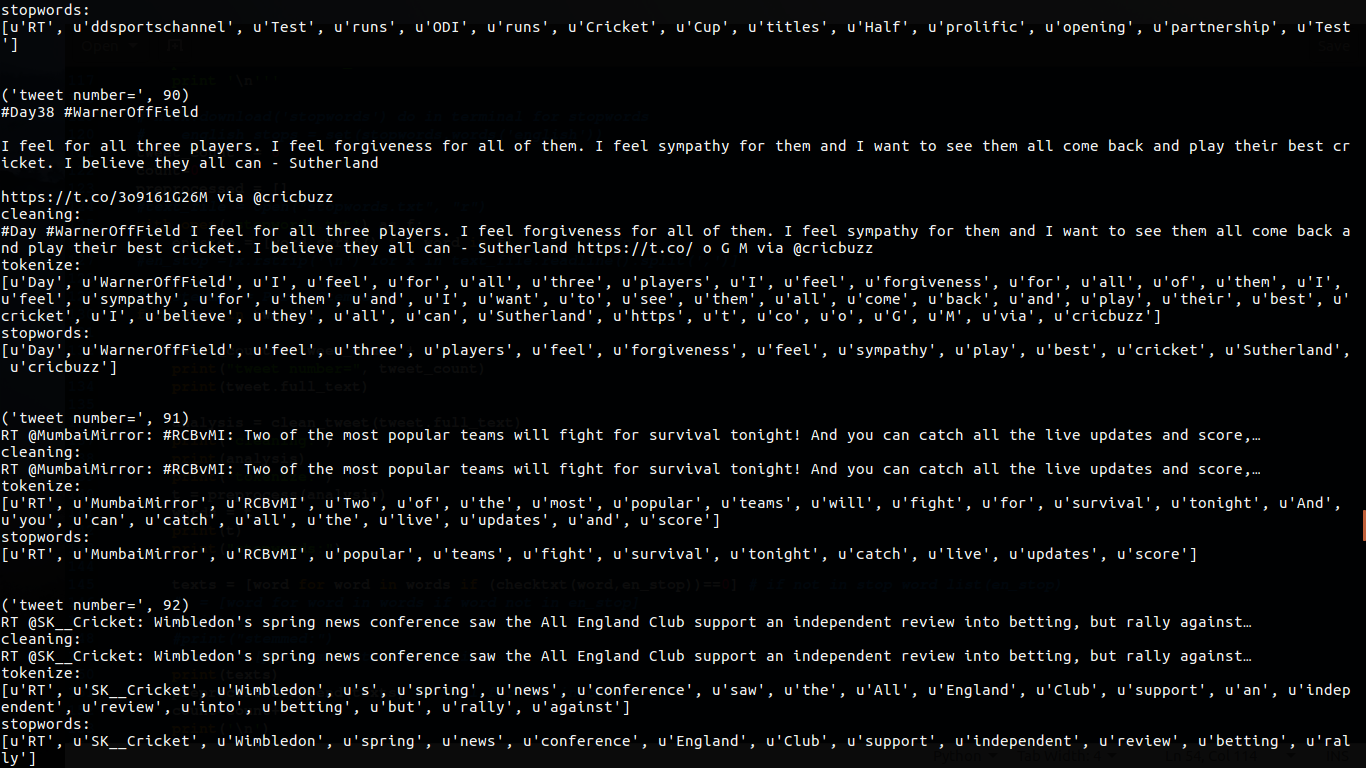
\includegraphics[width=0.9\linewidth]{preprocess.png}
	\caption{Output after preprocessing}
	\label{fig:expression01}
\end{figure}


\end{itemize}
\subsection{REPRESENTING DATA}
For training the tweets needed to be represented in the form which would be understandable by the machine. Thus \textbf(LIBLINEAR REPRESENTION was used to represent tweets . To convert tweets to  LIBLINEAR format,\textit(BAG-OF-WORDS) concept was used . It consists of 2 dictionaries.
\begin{itemize}
	\item Word - ID DIctionary
	\item Tweet - Category Dictioniary

\end{itemize}
\paragraph{}
The WORD-ID  dictionary converts each word in the tweet into a unique id. This dictionary is a  common throughout the project. Each word is assigned an unique id in the order of their arrival .  This dictionary is stored as text file and maintained.
The format being - $<$WORD$>$ $<$WORDID$>$
\begin{figure}[h]
	\centering
	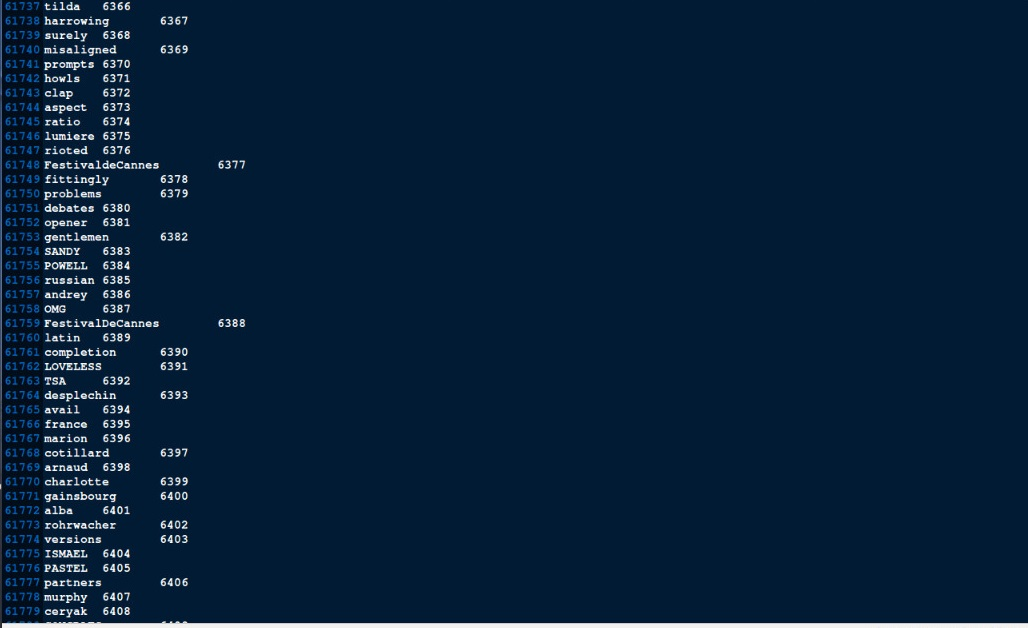
\includegraphics[width=0.9\linewidth]{word.jpg}
	\caption{Word dictionary containing a unique index for each of the words occurring in the tweets present in the training data set}
	\label{fig:expression01}
\end{figure}
\paragraph{}The TWEET -Category Dictionary is a mapping from tweet - Wordset dictionary to its category ID. The category id was explicitly given in a particular order. The order being :
\begin{itemize}
	\item 1.  SPORTS
	\item 2.  FINANCE
	\item 3.  POLITICS
	\item 4.  TECHNOLOGY
	\item 5.  ENTERTAINMENT
\end{itemize}
The tweets collected in each category were preprocessed and was stored in Tweet - Category Dictioniary . Each word belonging to which tweet Id and category were specified. The format of this dictionary being:
$<$Category ID$>$ $<$Tweet ID$>$ $<$ Word ID $>$ $<$ Value $>$
Value was always given as 1.

\begin{figure}[!ht]
	\centering
	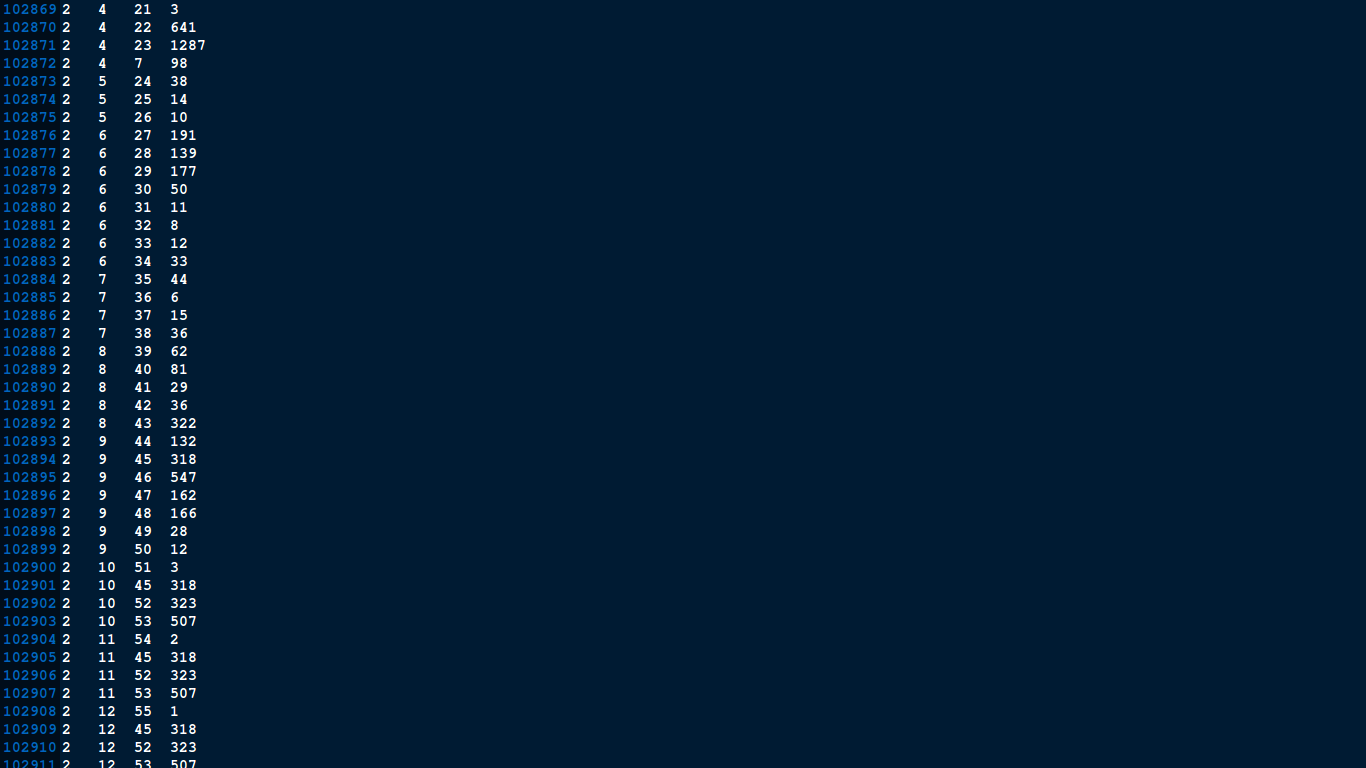
\includegraphics[width=0.9\linewidth]{document_file.png}
	\caption{Tweet category dictionary}
	\label{fig:expression01}
\end{figure}


\paragraph{}
The Tweet - category dictionary was used in generation of the LIBLINEAR representation . The format of LIBLINEAR is :\\
\linebreak
$<$\textbf{category Id}$>$ $<$\textbf{Feature ID 1}$>$:$<$\textbf{Value}$>$ $<$\textbf{Feature ID 2}$>$:$<$\textbf{Value}$>$... \\
$
. \\
. \\
$
$<$\textbf{category Id}$>$ $<$\textbf{Feature ID 1}$>$:$<$\textbf{Value}$>$ $<$\textbf{Feature ID 2}$>$:$<$\textbf{Value}$>$...
\linebreak
\linebreak
Each line in the represents tweet, each feature represents a word. Each value represents the weight of the feature. \\
\linebreak
Each category creates a liblinear text file and is saved to provide it as an input to the classifier. The text files are saved in the same namme as that of the categories

\begin{figure}[!ht]
	\centering
	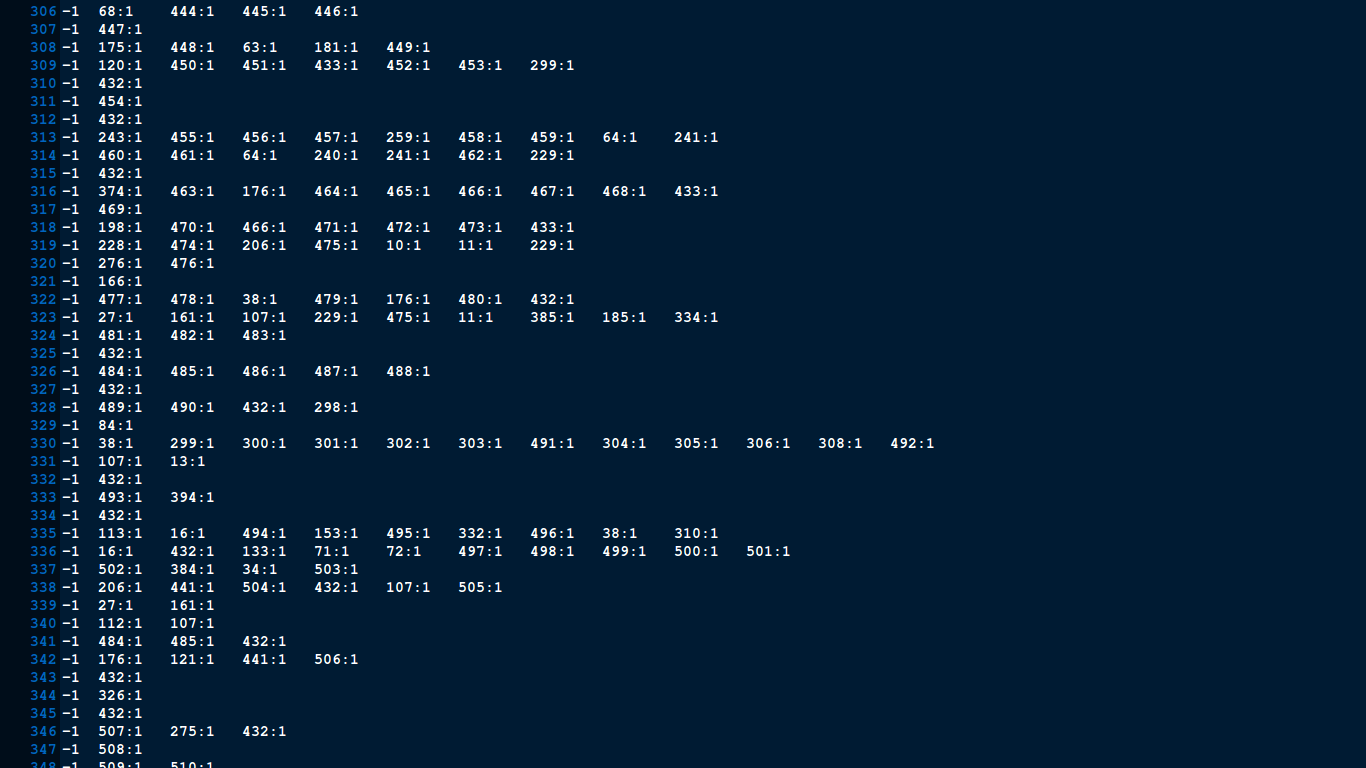
\includegraphics[width=0.9\linewidth]{liblinear.png}
	\caption{Liblinear format}
	\label{fig:expression01}
\end{figure}

Upon testing a new user's tweet the same procedures are repeated except on unlabelling the tweets. Here the category id is asssigned 0 . This indicates that these tweets needed to be classified .
\subsection{SVM CLASSIFIER}
\textbf{Training:}
For the purposes of classification, multiclass linear  classifiers were used. In tweet classification , the features used are words. Hence the feature representations need to be done appropriately. For this purpose , LIBLINEAR Representations were used.  SVM uses mathematical calculations and Vector multiplication for classification. Thus words need to be converted into numerical values. This was done by creating dictionaries and mapping them properly.
\paragraph{}
  Thus, the classifier had to classify into: Sports, Finance, Entertainment, Technology and  Politics. For this purpose, we 5 One vs. Rest classification models were created, one for each  category.
 
 
In One Vs Rest is implented by creating the LIBLINEAR file accordingly. The tweets belonging to the respective categories were assigned the category ID. The rest of the tweets were categorized as -1. This is essential because the classifier need to learn negative values too. Thus each file had both positive and negative tweets .
\paragraph{}

 

 
 \paragraph{}
  After the training process each category creates and saves its model . Thus 5 models are created to the respetive categories . This model is given as an input to the classifier . 
  \paragraph{} 
  \textbf{Testing:}
  Each tweet is passed through each of these classifier models. The output of each  of these classifiers would be whether the tweet belongs to the  category that classifier is trained for or not . Thus, after the tweet has passed  through all the five  classifiers, the categories in which the user has maximum interest is obtained . The percentage of his interesrts in other categories are also obtained .

\section{SENTIMENT ANALYSIS}
\paragraph{}
Opinion mining or sentiment analysis refers to the use of natural language processing, text analysis, computational linguistics, and biometrics to systematically identify, extract, quantify, and study affective states and subjective information.

Sentiment analysis is widely applied to voice of the customer materials such as reviews and survey responses, online and social media, and healthcare materials for applications that range from marketing to customer service to clinical medicine.


\subsection{DATA COLLECTION FOR SENTIMENT ANALYSIS}
The input search word, location name and the range in km are taken as input from the user. The location name is converted to corresponding lattitude and longitude, the search word, lattitude and longitude and range in km are given as input to tweepy. The tweets from the corresponding location about the particuar topic are returned. 

\subsection{PREPROCESSING}
Steps in preprocessing
\begin{itemize}
	\item{\textbf{Tokenization :}} Tokenization is the process of splitting up a string into a list of tokens and constructing a bag-of-words and is the first step of pre-processing. It involves splitting the text with white spaces to form a list of individual words in each text.
	
	\item{\textbf{Removing stop words :}} Stop-words such as articles, prepositions and short functionwords carry a connecting function in the sentence and have a high frequency of occurrence in the text. They can be removed from a bag-of-words since they do not affect the final sentiment of the text. This can be done by checking each word from the text against a dictionary including stop words such as “and”, “or”, “still”, “also”, “able”, “the”, “as”, “which” etc. and removing all the matching ones.
	
	\item{\textbf{Special symbols :}}  There are some symbols which may be used in tweets,for example the word following after the “@” symbol is a username and “hash” is used to mark topics
	or keywords in a tweet. All usernames and URLs were converted to generic tags (e.g. all @usernames tagged as “username”), and some mentions can be used to improve the performance of the sentiment classifier.
	
	\item{\textbf{Stemming :}}	Stemming is a technique used to remove affixes from a word replacing them with their roots reducing different forms of a word such as nouns,verbs, adjectives etc. to a common base form. (e.g. the words “analysis”, “analyzed”, “analyzing” and all other types of this word are converted to “analyse” after stemming).It helps to reduce the dimensionality of the bag-of-words and improves the output of sentiment classification.
	
\end{itemize}
\subsection{FEATURE EXTRACTION}
Selecting a useful list of words as features of a text. Or simply eliminating the words
that do not contribute to the text’s sentiment is called feature extraction. \\
The different methods of feature extraction are \\ \\
\textbf{Unigram feature :} Unigrams are the simplest method of feature extraction and
are defined as looking at one word at a time in a text, which can be extended to an
N-gram in order to exploit the ordering of words. It can be used in different states
of text such as characters, words or sentences. The unigrams were taken for analysis.

\subsection{SENTIMENT POLARITY CLASSIFIER}
 Sentiment polarity classification involves finding the polarity associated with the sentence or tweet. Dictionary based approach was used to analyse the the polarity of the sentence.
\subsubsection{DICTIONARY BASED APPROACH}
The Dictionary Approach uses a pre-built dictionary which defines semantic orientation
of words, such as the SentiWordNet, which is the standard dictionary today. Existing opinion mining approaches use these dictionaries mainly for identifying semantic orientation of
opinion words. Semantic orientation of a single sentence or review is generally calculated
by averaging the semantic orientation values of individual words. For instance, most of
the dictionary base methods aggregate the semantic orientation values for a sentence or
whole review, and estimate the resultant polarity using simple rule-based algorithms.
Each term in the microphrase is checked in the dictionary. The dictionary contains the
terms along with their polarity. A sentiment value of a review is computed by summing
the sentiment values of all opinion words occurring in the review. The resultant semantic
orientation value of a review shows its corresponding polarity, that is, greater than 0 for
positive, equal to 0 for neutral and less than 0 for negative. \\ \\
Examples of dictionaries are SentiWordNet, WordNetAffect, SenticNet, MPQA etc.

\subsubsection{MICROPHRASE}
\paragraph{} A statement or text will be sometimes divided into two or more subtexts or sub statements, these sub texts are termed as microphrase. Splitting cues divide the text into microphrases. A splitting cue can be an adverb, a conjunction or a punctuation. The total sentment orientation(SO) of the text will be sum of the sentiment polarities of the individual microphrases.
\\ \\
Example : "\textit{I dont like this phone, it's useless}"

here I dont like this phone is the first microphrase m1 
, is the splitting cue which divides the sentence 
it's useless is the second microphrase m2
\\ \\
The polarity of the textual content depends on the sum of polarities which compose it.
$$
% \begin{equation}
Pol(T) = \sum_{i=1}^{k} Pol(m_i)  , \hspace{1cm} where\hspace{0.2cm} T={m_1...m_k} \hspace{1cm} 
%\end{equation}
$$
%The polarity  of  the  microphrase depends on the polarity(score) of %the terms which compose it.
\\
\begin{equation}
Pol(m_i) = \sum_{j=1}^{n} Score(t_j) ,\hspace{1cm} where\hspace{0.2cm} m_i={t_1...t_n} \hspace{1cm}
\end{equation} 


The polarity  of  the  microphrase depends on the polarity(score) of the terms which compose it.


\subsubsection{CONJUNCTION RULES}
\paragraph{} The conjunction divide the statement into two or more microphrases. The two conjunctions used are \textbf{AND} and \textbf{BUT}.
\subsubsection{AND conjunction}
\paragraph{} If AND conjunction is used then the microphrases will have same polarity. That is both the microphrases will have either positive or negative value. \\
i.e  If $ m_1 $ AND $ m_2 $ are the microphrases
then $ m_1 $ and $ m_2 $ will have same polarity
\\ \\
Example : "The phone a has better camera \textbf{and} a good battery"
\\
Here the first micro phrase and second micro phrase has positive polarity.
\subsubsection{BUT conjunction}
\paragraph{} If BUT conjunction is used then the microphrases will have opposite polarity. That is if one microphrase has a positive polaity the other will have a negative polarity and vice versa.
\\
i.e If $ m_1 $ BUT $ m_2 $ are the microphrases then $ m_1 $ and $ m_2 $ will have opposite polarity.
\\ \\
Example : "The voice quality of this phone is not good, but the  battery life is long"
\\
Here the first microphrase has a negative polarity and the second microphrase has a positive polarity.

\subsubsection{SHIFT IN OPINION SENTIMENT POLARITY}
\paragraph{}The polarity of the sentiment words are altered when certain words are  present before the sentiment words. The words not, ain't etc reverses the polarity, these words are called negators. Certain words like so, great, huge, pretty etc increase or decrease the magnitude of the sentiment orientation, these words are called intensifiers. 
\subsubsection{NEGATION}
\paragraph{}  Negators are words which reverses the polarity of the sentiment word which comes after it, example changing good (+2)
into not good (-2). (e.g. no, not, neither, nor, nothing, never,
none) are very important in identifying the sentiments
A backward search is required to find the negators.
\\
Examples of negators are not, none, nobody, never and nothing.
\begin{equation}
% $$ 
W_s = W_s * (-1), \hspace{1cm} W_s  \hspace{0.1cm}is \hspace{0.1cm}  word \hspace{0.1cm} sentiment
%\hspace{1cm}
\end{equation}
% $$ \hspace{0.2cm}
\\
Eg :- \textbf{Nobody} gives a good performance in this movie.
\\
Negation is one of the most common linguistic means that can change text polarity. Therefore in sentiment analysis negation has to be  taken into account. The  scope size of a negation expression determines which sequence of words in the sentence is affected by negation words, such as, no, not, never. Negation terms affect the contextual polarity of words but the presence of a negation  word  in  a  sentence  does  not  mean that  all of the words conveying sentiments willbe  inverted.

%\renewcommand\chaptername{CHAPTER}
\subsubsection{INTENSIFICATION}
\paragraph{} Intensifiers either amplifies (increases) or decreases the semantic intensity of a neighbouring lexical item.
Intensifiers use simple addition and subtraction 
Intensifers are usually expressed in precentage
$$
W_s = (100 + S_{inf}) * O_s   \hspace{1cm}
W_s \hspace{0.1cm} is\hspace{0.1cm} word \hspace{0.1cm} sentiment\\ $$ 
$ S_{inf} $ is intensifier value in percentage and $ O_s $ is the score of opinion word.
\\  \\
Intensifiers can be cassified into two categories, depending on their polarity: Amplifiers increase the semantic intensity of the neighbouring lexical item, whereas downtoners decrease it. The intensification is modeled using modifiers, with each intensifying word having a percentage associated with it, amplifiers are positive, whereas downtoners are negative.
\\
For example, if \textit{sleazy} has an SO value of -3 \textit{somewhat sleazy} would have an SO value of: $ -3*(100-30)/100 = -2.1 $. 
If excellent has a SO value of 5, most excellent would
have an SO value of:$ 5 * (100 + 100) = 10$. Intensifiers are applied recursively starting from the closest to the SO-valued word: If good has an SO value of 3, then really very good has an SO value of $ (3 * [100 + 25]) *(100 + 15) = 4 $.Because our intensifiers are implemented using a percentage scale, they are able to fully capture the variety of intensifying words as well as the SO value of the item
being modified. This scale can be applied to other parts of speech, given that adjectives, adverbs, and verbs use the same set of intensifiers.


\subsubsection{DICTIONARIES USED}
\begin{itemize}
	\item \textbf{Sentiment Orientation dictionary} \\
	A sentiment polarity dictionary consisting of all sentiment words along with their polarities was used. Over 7000 words along with their polarities were represented.
	\item \textbf{Negator dictionary} \\
	A dictionary consisting of all negators were used. The negators along with a flag with value 1 was represented in the negator dictionary. The flag value indicates the word is a negator.
	\item \textbf{Intensifier dictionary} \\
	A dictionary of intensifier words along with their degree of intensification was used. The degree of intensification was represented in percentage. The intensifier word is the key and the degree of intensification is the value.

\end{itemize}
All the dictionaries were represented as hash tables for faster search and retrival. The python dictionary data structure was used for its representation.
\subsubsection{DATA STRUCTURE USED}
\subsubsection{HASH TABLE}
hash table (hash map) is a data structure which implements an associative array abstract data type, a structure that can map keys to values. A hash table uses a hash function to compute an index into an array of buckets or slots, from which the desired value can be found.

Ideally, the hash function will assign each key to a unique bucket, but most hash table designs employ an imperfect hash function, which might cause hash collisions where the hash function generates the same index for more than one key. Such collisions must be accommodated in some way. Thus the goal is to design a hash function that has least collisions.

In a well-dimensioned hash table, the average cost (number of instructions) for each lookup is independent of the number of elements stored in the table. Many hash table designs also allow arbitrary insertions and deletions of key-value pairs.

The dictionaries were represented in hash tables. The python dictionary data type was used to create the hash tables.

The use of hash table resulted in a time complexity of $ O(1) $ for search and retrieval of  sentiment polarity of the words.
\\

\begin{figure}[!ht]
	\centering
	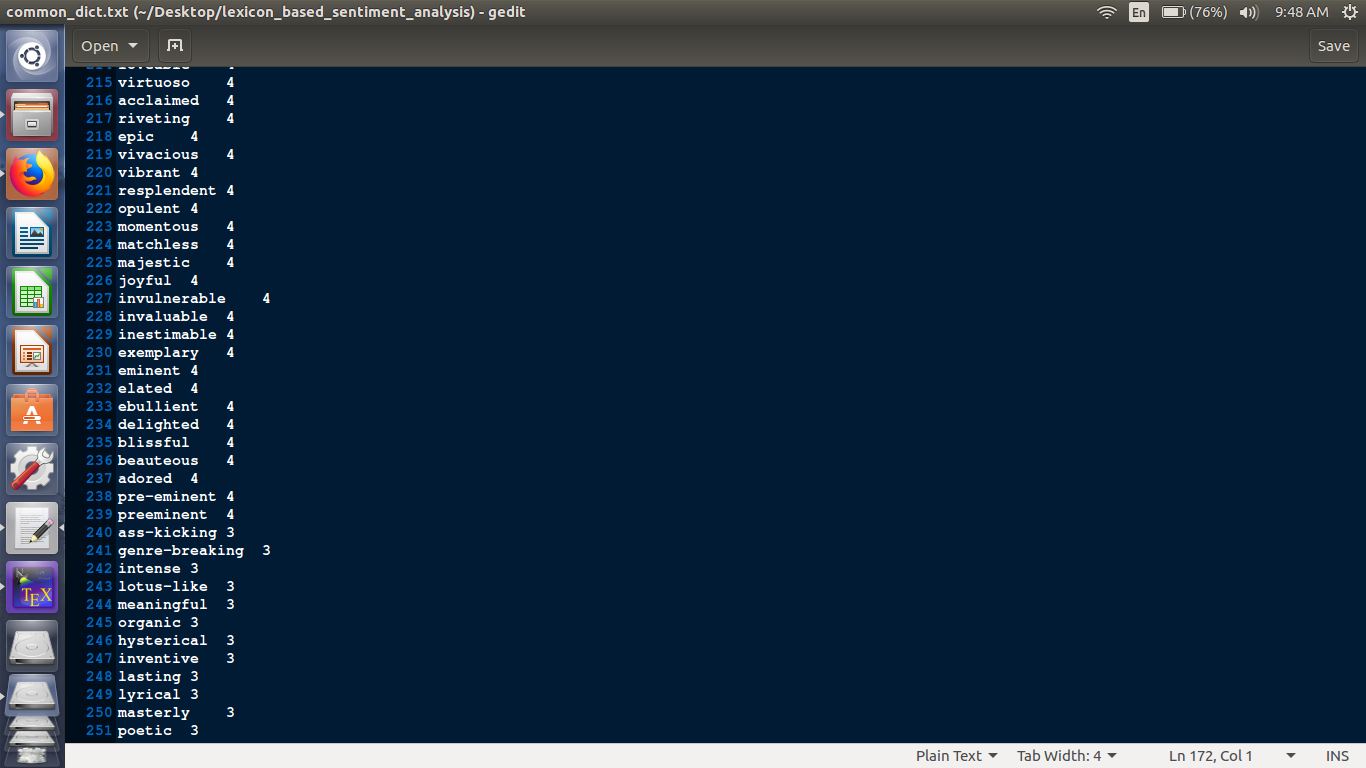
\includegraphics[width=0.8\linewidth]{common_dict1.png}
	\caption{Sentiment dictionary positive words}
	\label{types}
\end{figure}
\begin{figure}[!ht]
	\centering
	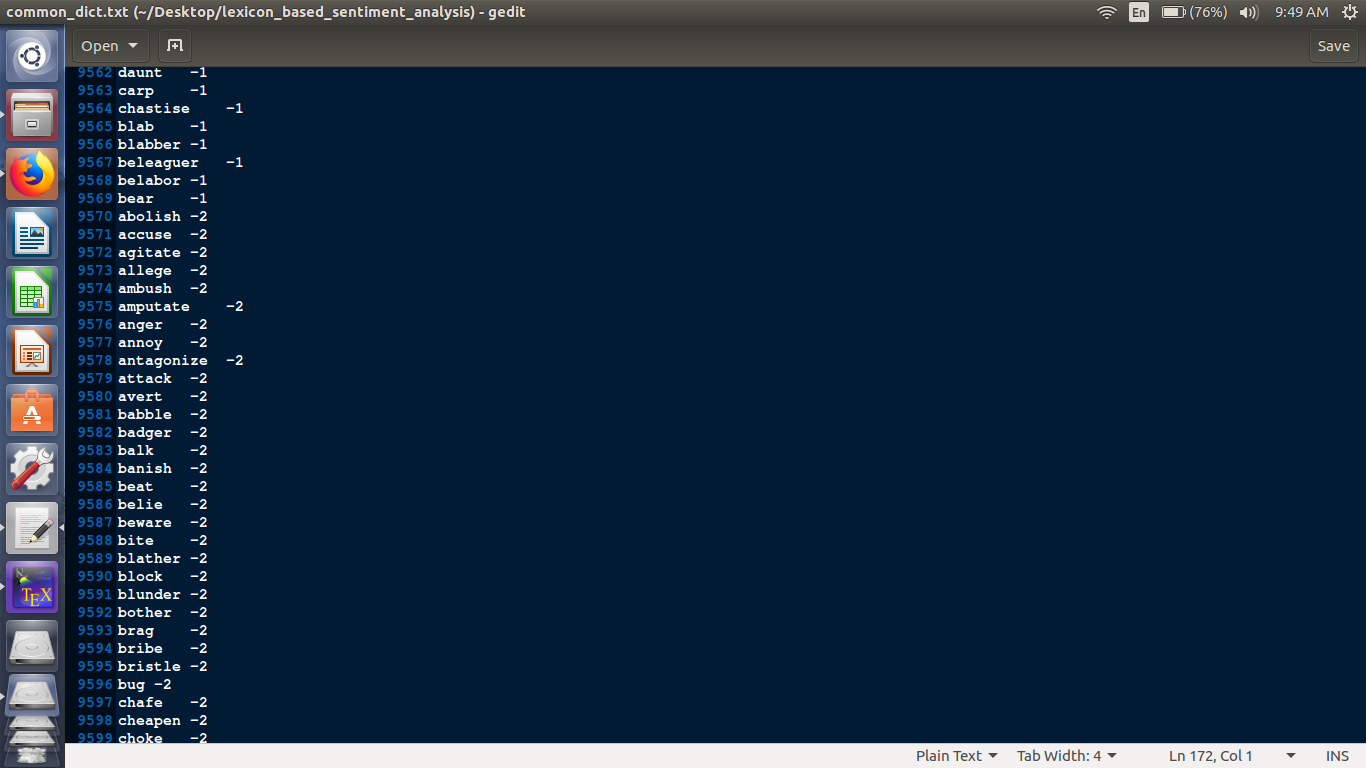
\includegraphics[width=0.8\linewidth]{common_dict2.png}
	\caption{Sentiment dictionary negative words}
	\label{types}
\end{figure}


\renewcommand\chaptername{CHAPTER}
\chapter{OUTPUT}
\subsection{Sentiment analysis}
\paragraph{} The percentage of positive, negative and neutral tweets were represented in the form of a pie chart. The percentage distribution of positive, negative and neutral tweets were given to the webpage. The pie chart is then plotted for these values. The accuracy of the system is 83 percent.
\\
\subsection{Topic modelling}
\paragraph{} The percentage of tweets from categories Sports, Finance, Politics, Technology and Entertainment were represented in the form of a pie chart. The percentage tweet distribution from individual categories were given to the webpage. The pie chart is then plotted for these values. The accuracy of the system was observed to be 78 percent.

\begin{figure}[!ht]
	\centering
	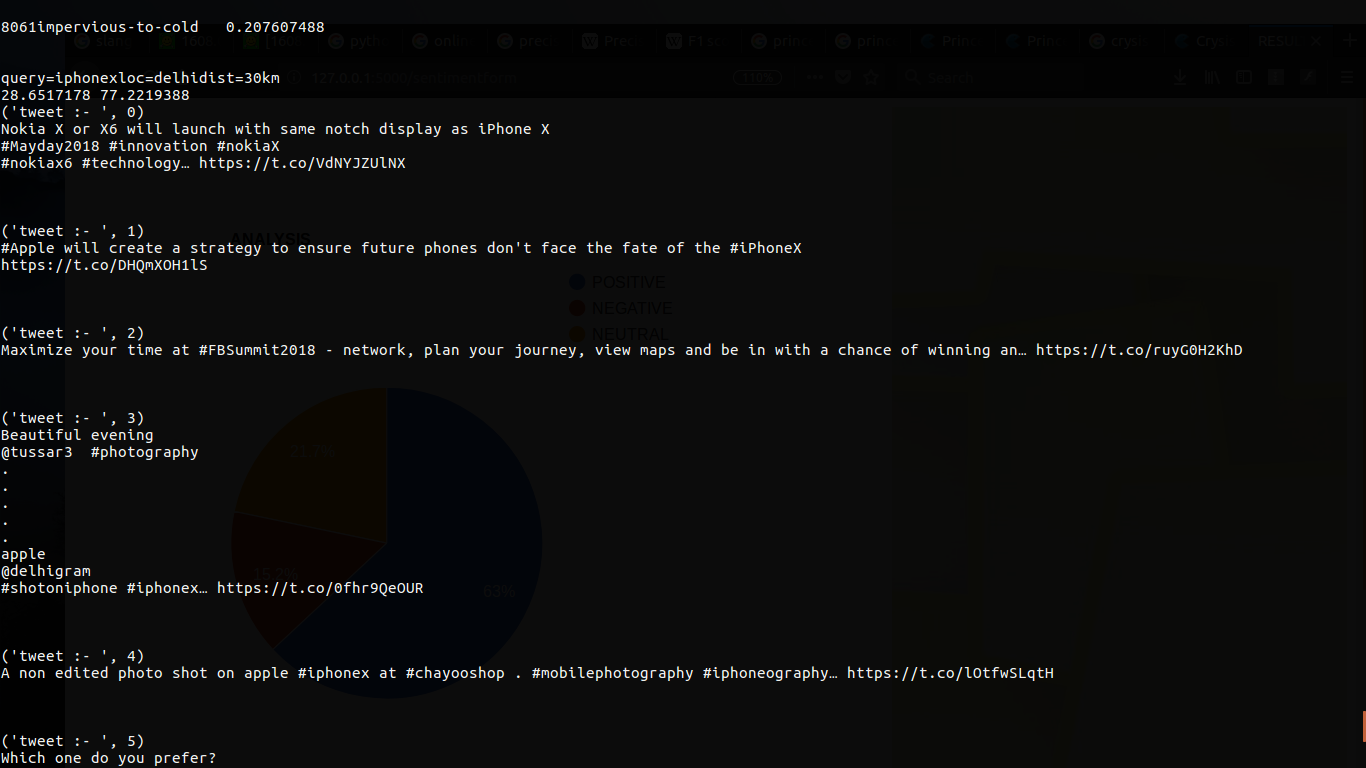
\includegraphics[width=0.9\linewidth]{sentiment_server.png}
	\caption{Sentiment analysis tweet collection}
	\label{fig:expression01}
\end{figure}


\begin{figure}[h]
	\centering
	
\includegraphics[width=0.9\linewidth]{image1.png}
	\caption{Front end screenshot 1}
	\label{fig:expression01}
\end{figure}

\begin{figure}[h]
	\centering
	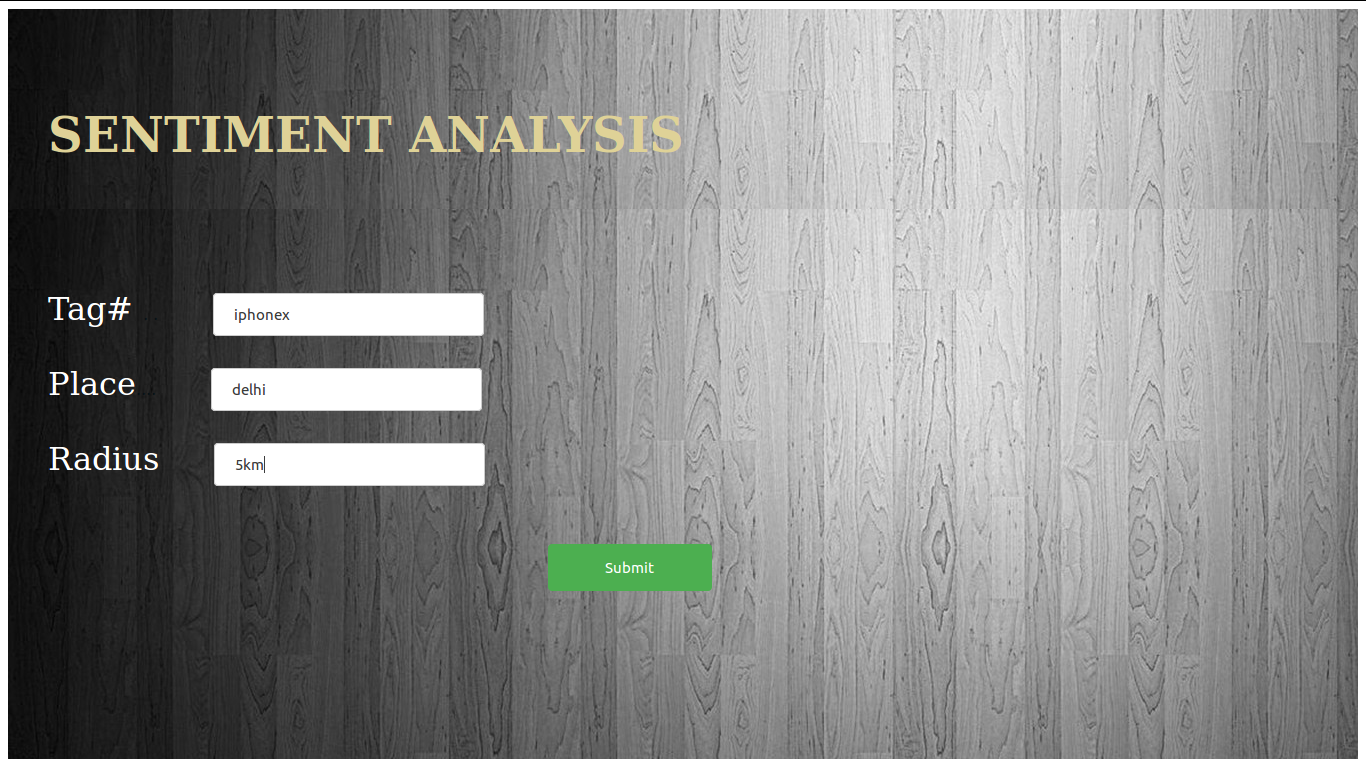
\includegraphics[width=0.9\linewidth]{image2.png}
	\caption{Front end screenshot 2}
	\label{fig:expression01}
\end{figure}

\begin{figure}
	\centering
	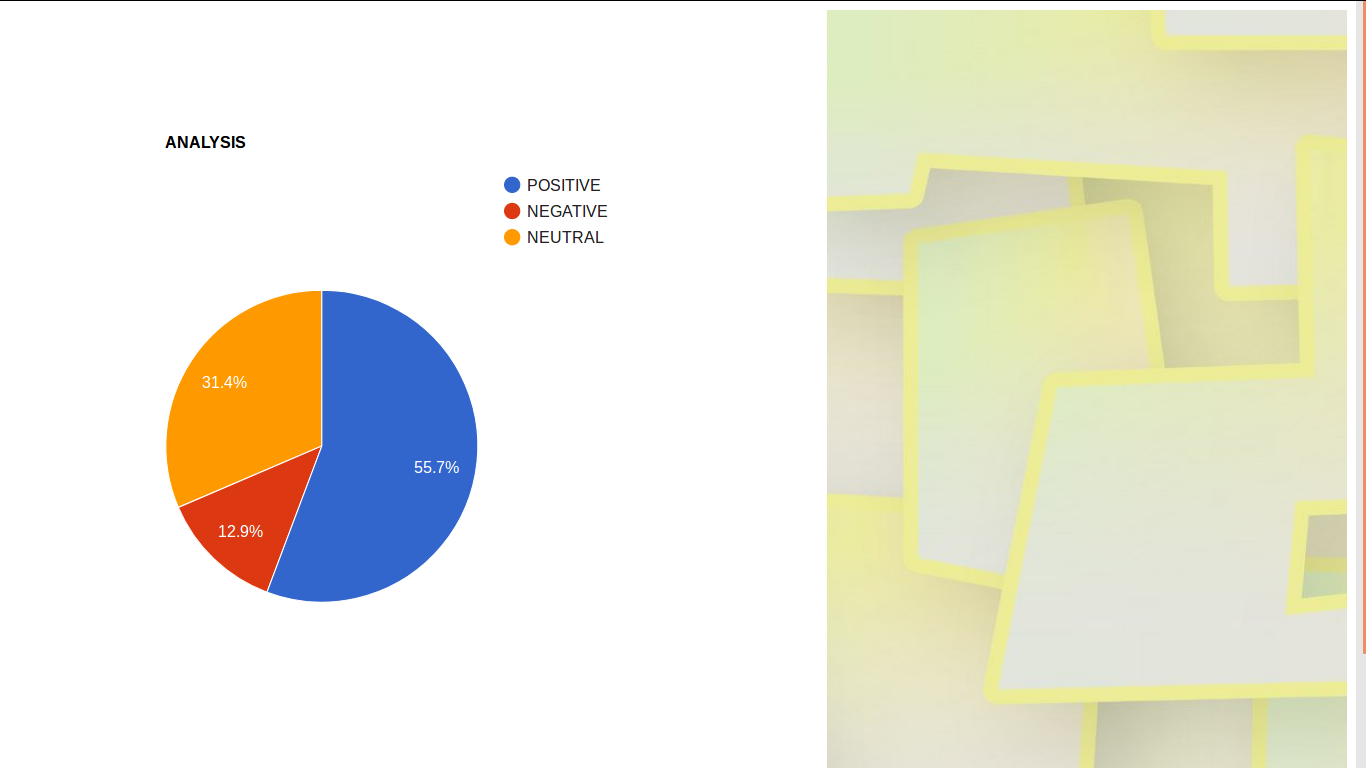
\includegraphics[width=0.8\linewidth]{new_out_sent.png}
	\caption{Output}
	\label{types}
\end{figure}

\begin{figure}[h]
	\centering
	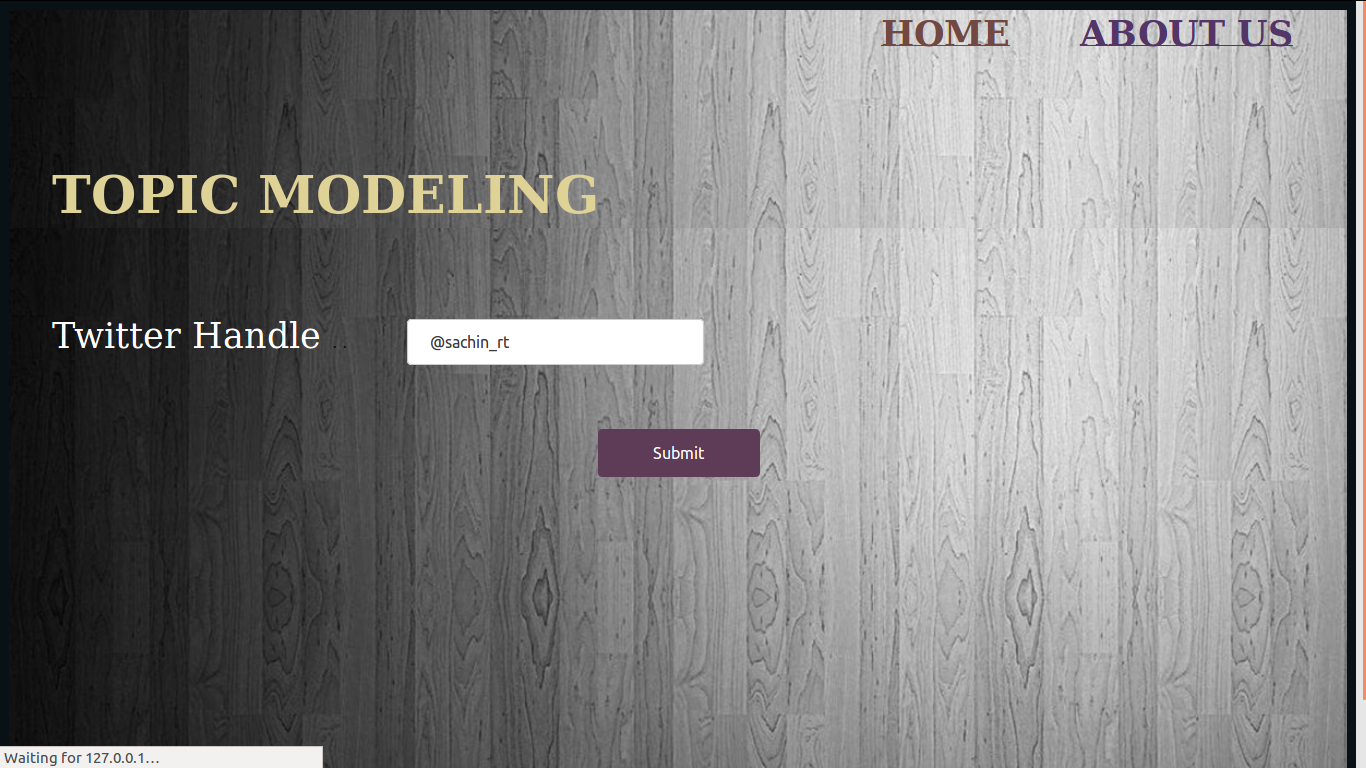
\includegraphics[width=0.9\linewidth]{sachin_topic.png}
	\caption{Front end screenshot 3}
	\label{fig:expression01}
\end{figure}

\begin{figure}[h]
	\centering
	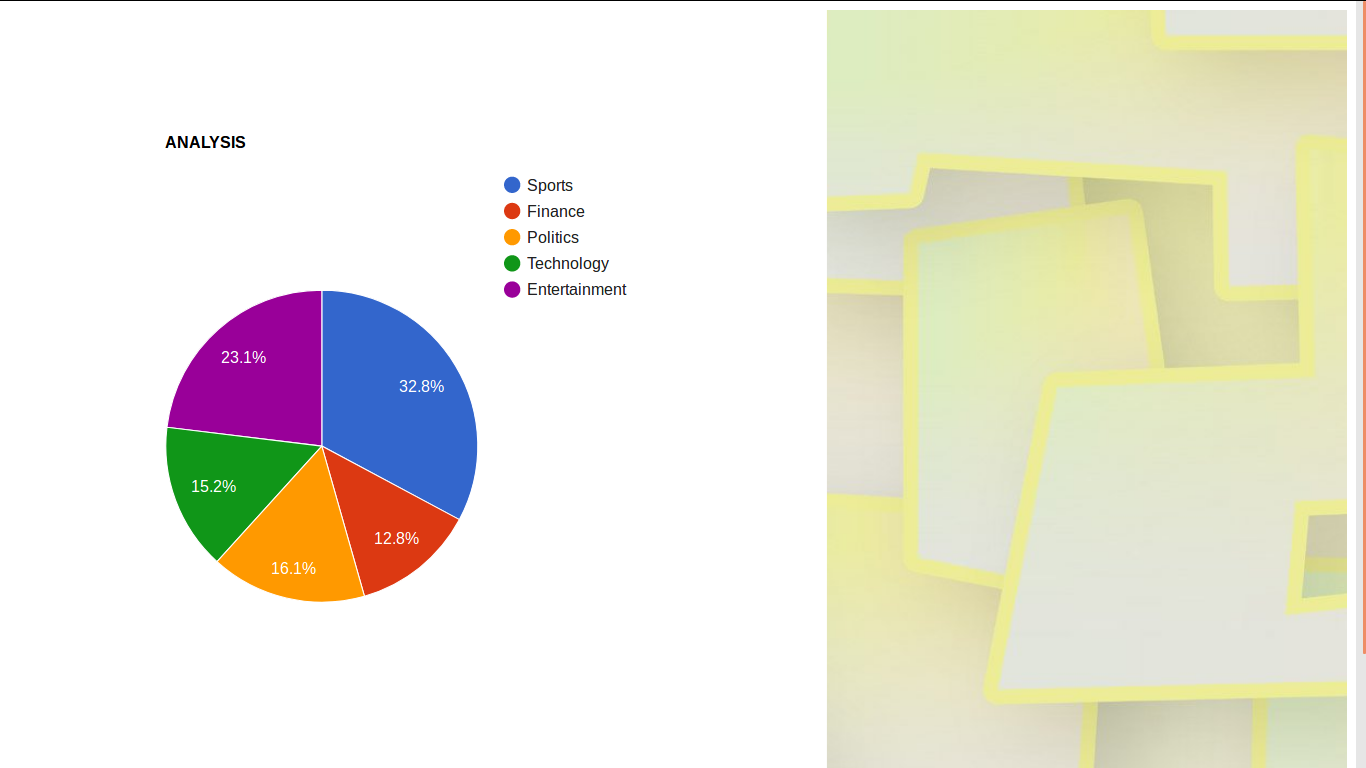
\includegraphics[width=0.9\linewidth]{sachin_topic_1.png}
	\caption{Output of topic modeling}
	\label{fig:expression01}
\end{figure}


\chapter{CONCULSION}

\paragraph{}
The project attempts to identify the interests of a given user as well as the sentimnents of various users on a particular topic. Classifier module using supervised machine learning techniques were used in identifying specific user interests.Increasing the size of the training dataset further added to improvement in the overall precision and recall. Lexicon-based sentiment analysis of a given topic were also  obtained.The sentiment scores of individual tweets were aggregated to compute the percentage of tweets in each class positive,negative or neutral. The final output was plotted as a pie graph in a web page. 

\paragraph{}
The system can be used for targeted ads to users by identifying their interests. As affliate marketing became common with the advent of social networking sites, the project offers a way of identifying the various interests of users to accurately target them with ads and affiliate marketing links.

The location based sentiment analysis can be used for analysing the user opinions about any products in the region to efficiently target the ads to them.
 
\chapter{FUTURE WORK}
\section{Sentiment analysis}
	\paragraph{} The main problem with social networking sites is the extensive use of slang words and emoticons. Thus accuracy of the system can be improved by including emoticon and slang word dictionaries. In this case the preprocessing should be carefully done so that the emoticons and slang words are not removed. Spam detection can be added to improve the accuracy of the result. The system is very useful for identifying the user opinions of products, this analysis can be used for targeting the particular users wtih ads and affiliate marketing links
	
\section{User interest identification}
	\paragraph{} the accuracy of the user interest identification system can be increased by expanding the link with a short summary of the content, therby using the links rather than simply eliminating it. A hirarchical analysis can be done to extract maximum information. That is within each category a hirarchical analysis can be done to analyze the entities or topics that the user is interested in each category. Furthermore the number of categories can be increased.
	
\chapter{REFERENCES}
\begin{enumerate}
\item[[ 1]]{ Rong-En Fan Kai-Wei, Chang Cho-Jui Hsieh, Xiang-Rui Wang, Chih-Jen Li "LIBLINEAR: A Library for Large Linear Classification "http://jmlr.csail.mit.edu/
papers/volume9/fan08a/fan08a.pdf}

\item[[ 2]]{  Chih-Wei Hsu, Chih-Chung Chang, and Chih-Jen Lin "A practical guide to libSVM" http://www.csie.ntu.edu.tw/~cjlin/papers/guide/guide.pdf}

\item[[ 3]]{ Yi Liu and Y. F. Zheng, "One-against-all multi-class SVM classification using reliability measures," Proceedings. 2005 IEEE International Joint Conference on Neural Networks, 2005., 2005, pp. 849-854 vol. 2.
doi: 10.1109/IJCNN.2005.1555963}

\item[[ 4]]{ R. Wang, S. Kwong and D. G. Chen, "A new method for multi-class support vector machines by training least number of classifiers," 2011 International Conference on Machine Learning and Cybernetics, Guilin, 2011, pp. 648-653.
doi: 10.1109/ICMLC.2011.6016830}

\item[[ 5]]{ G. Madzarov and D. Gjorgjevikj, "Multi-class classification using support vector machines in decision tree architecture," IEEE EUROCON 2009, St.-Petersburg, 2009, pp. 288-295.
doi: 10.1109/EURCON.2009.5167645}

\item[[ 6]]{Solanki Yogesh,	S. Y. Ganeshbhai and B. K. Shah, "Feature based opinion mining: A survey," 2015 IEEE International Advance Computing Conference (IACC), Banglore, 2015, pp. 919-923.	
}
\item[[ 7]] { K. Z. Aung and N. N. Myo, "Sentiment analysis of students' comment using lexicon based approach," 2017 IEEE/ACIS 16th International Conference on Computer and Information Science (ICIS), Wuhan, 2017, pp. 149-154.
	doi: 10.1109/ICIS.2017.7959985}

\item[[ 8]] {Peiman Barnaghi and John G. Breslin and Parsa Ghaffari, “Opinion Mining and Sentiment Polarity on Twitter and Correlation Between Events and Sentiment”, 2016 IEEE Second International Conference on Big data Computing Service and Applications
}

\end{enumerate}
